% ============================================================
% Figure 1: DEAC System Overview (Main Block Diagram)
% ============================================================
\documentclass[border=5pt]{standalone}
\usepackage[T1]{fontenc}
\usepackage{tikz}
\usetikzlibrary{arrows.meta, positioning, shapes.geometric, fit, calc, decorations.pathreplacing, backgrounds}

% IEEE Colors (colorblind-safe)
\definecolor{cb1}{RGB}{0,101,189}     % Blue
\definecolor{cb2}{RGB}{204,51,51}     % Red
\definecolor{cb3}{RGB}{0,128,0}       % Green
\definecolor{cb4}{RGB}{230,159,0}     % Orange
\definecolor{cb5}{RGB}{117,112,179}   % Purple
\definecolor{cbg}{RGB}{240,240,240}   % Light gray

\begin{document}
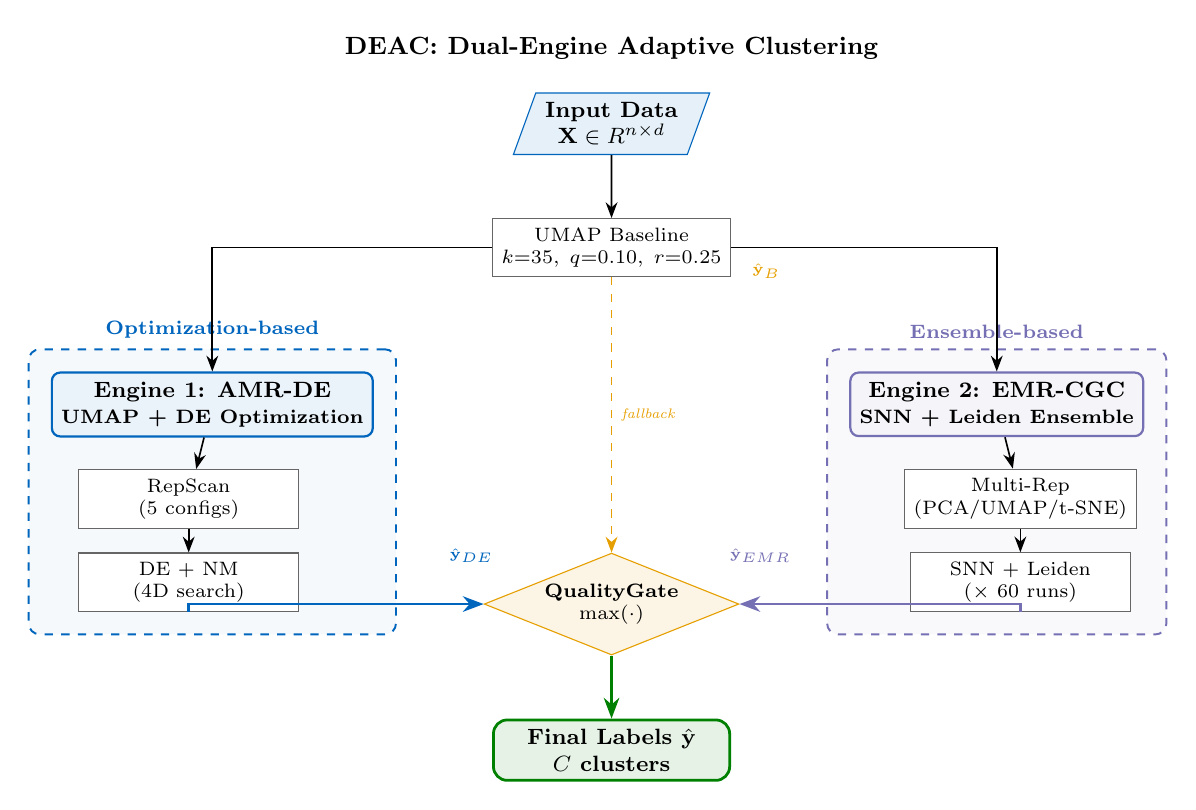
\begin{tikzpicture}[
    >=Stealth,
    node distance=0.6cm and 1.2cm,
    font=\footnotesize,
    % Styles
    input/.style={trapezium, trapezium left angle=70, trapezium right angle=110,
        draw=cb1, fill=cb1!10, minimum width=2.5cm, minimum height=0.6cm,
        align=center, font=\footnotesize\bfseries},
    engine/.style={rectangle, rounded corners=3pt, draw=#1, fill=#1!8,
        minimum width=3.5cm, minimum height=0.7cm, align=center,
        font=\footnotesize\bfseries, line width=0.8pt},
    process/.style={rectangle, draw=black!60, fill=white,
        minimum width=2.8cm, minimum height=0.55cm, align=center,
        font=\scriptsize},
    decision/.style={diamond, aspect=2.5, draw=cb4, fill=cb4!10,
        minimum width=1.5cm, font=\scriptsize\bfseries, align=center,
        inner sep=1pt},
    output/.style={rectangle, rounded corners=5pt, draw=cb3, fill=cb3!10,
        minimum width=3cm, minimum height=0.7cm, align=center,
        font=\footnotesize\bfseries, line width=1pt},
    groupbox/.style={rectangle, rounded corners=4pt, draw=#1, dashed,
        fill=#1!4, inner sep=8pt, line width=0.7pt},
    arr/.style={-Stealth, line width=0.6pt},
    thickarr/.style={-Stealth, line width=1pt, #1},
]

% ── Input ──
\node[input] (input) {Input Data\\$\mathbf{X} \in \mathbb{R}^{n \times d}$};

% ── Baseline ──
\node[process, below=0.8cm of input] (baseline) {UMAP Baseline\\$k{=}35,\; q{=}0.10,\; r{=}0.25$};

% ── Two Engines ──
\node[engine=cb1, below left=1.2cm and 1.5cm of baseline] (amr) {Engine 1: AMR-DE\\{\scriptsize UMAP + DE Optimization}};
\node[engine=cb5, below right=1.2cm and 1.5cm of baseline] (emr) {Engine 2: EMR-CGC\\{\scriptsize SNN + Leiden Ensemble}};

% ── Engine 1 sub-steps ──
\node[process, below=0.4cm of amr, xshift=-0.3cm] (amr1) {RepScan\\(5 configs)};
\node[process, below=0.3cm of amr1] (amr2) {DE + NM\\(4D search)};

% ── Engine 2 sub-steps ──
\node[process, below=0.4cm of emr, xshift=0.3cm] (emr1) {Multi-Rep\\(PCA/UMAP/t-SNE)};
\node[process, below=0.3cm of emr1] (emr2) {SNN + Leiden\\($\times$ 60 runs)};

% ── QualityGate ──
\node[decision, below=3.5cm of baseline] (qg) {QualityGate\\$\max(\cdot)$};

% ── Output ──
\node[output, below=0.8cm of qg] (out) {Final Labels $\hat{\mathbf{y}}$\\$C$ clusters};

% ── Group boxes ──
\begin{scope}[on background layer]
    \node[groupbox=cb1, fit=(amr)(amr1)(amr2), label={[cb1, font=\scriptsize\bfseries]above:Optimization-based}] {};
    \node[groupbox=cb5, fit=(emr)(emr1)(emr2), label={[cb5, font=\scriptsize\bfseries]above:Ensemble-based}] {};
\end{scope}

% ── Arrows ──
\draw[arr] (input) -- (baseline);
\draw[arr] (baseline) -| (amr);
\draw[arr] (baseline) -| (emr);
\draw[arr] (amr) -- (amr1);
\draw[arr] (amr1) -- (amr2);
\draw[arr] (emr) -- (emr1);
\draw[arr] (emr1) -- (emr2);
\draw[thickarr=cb1] (amr2) |- (qg);
\draw[thickarr=cb5] (emr2) |- (qg);
\draw[arr, dashed, cb4] (baseline) -- (qg) node[midway, right, font=\tiny\itshape] {fallback};
\draw[thickarr=cb3] (qg) -- (out);

% ── Labels on arrows ──
\node[font=\tiny, cb1, above left=0.1cm of qg, xshift=-0.5cm] {$\hat{\mathbf{y}}_{DE}$};
\node[font=\tiny, cb5, above right=0.1cm of qg, xshift=0.5cm] {$\hat{\mathbf{y}}_{EMR}$};
\node[font=\tiny, cb4, right=0.15cm of baseline, yshift=-0.3cm] {$\hat{\mathbf{y}}_{B}$};

% ── Title ──
\node[above=0.3cm of input, font=\small\bfseries] {DEAC: Dual-Engine Adaptive Clustering};

\end{tikzpicture}
\end{document}
